\documentclass{beamer}
\usetheme{Singapore}
\usepackage{changepage,amsmath}

%\usepackage{pstricks,pst-node,pst-tree}
\usepackage{amssymb,latexsym}
\usepackage{tikz}
\usepackage{graphicx}
\usepackage{fancyvrb}
\usepackage{hyperref}
\usepackage{fancybox}
\usepackage[listings]{tcolorbox}

\definecolor{codegreen}{rgb}{0,0.6,0}
\definecolor{codegray}{rgb}{0.5,0.5,0.5}
\definecolor{codepurple}{rgb}{0.58,0,0.82}
\definecolor{backcolour}{rgb}{0.95,0.95,0.92}

\lstdefinestyle{mystyle}{
    language=Python,
    backgroundcolor=\color{backcolour},   
    commentstyle=\color{codegreen},
    keywordstyle=\color{magenta},
    numberstyle=\tiny\color{codegray},
    stringstyle=\color{codepurple},
    basicstyle=\ttfamily\scriptsize,
    breakatwhitespace=false,         
    breaklines=true,                 
    captionpos=b,                    
    keepspaces=true,                 
    numbers=left,                    
    numbersep=5pt,                  
    showspaces=false,                
    showstringspaces=false,
    showtabs=false,                  
    tabsize=2,
    escapechar=|,
    frame=single
}

\lstset{style=mystyle}


\newcommand{\bi}{\begin{itemize}}
\newcommand{\li}{\item}
\newcommand{\ei}{\end{itemize}}
\newcommand{\Show}[1]{
\begin{center}
\shadowbox{\begin{minipage}{0.8\textwidth}
          #1
          \end{minipage}}
\end{center}
}
\newcommand{\arrow}{\ensuremath{\rightarrow}}

\newcommand{\uparr}{\ensuremath{\uparrow}}


\newcommand{\fig}[2]{\centerline{\includegraphics[width=#1\textwidth]{#2}}}

\newcommand{\bfr}[1]{\begin{frame}[fragile]\frametitle{{ #1 }}}
\newcommand{\efr}{\end{frame}}

\newcommand{\cola}[1]{\begin{columns}\begin{column}{#1\textwidth}}
\newcommand{\colb}[1]{\end{column}\begin{column}{#1\textwidth}}
\newcommand{\colc}{\end{column}\end{columns}}


\title{Fundamentals of Data Visualization}
\author{Chapter 3}

\begin{document}

\begin{frame}
\maketitle
\end{frame}

\bfr{Coordinate systems and axes}
\fig{.8}{cartesian-coord-1}


\end{frame}

\bfr{Choice of axes}
\fig{.8}{temperature-normals-Houston-1.png}


\end{frame}

\bfr{Choice of axes when both axes are the same quantity}
\fig{.8}{temperature-normals-Houston-San-Diego-1}

\bi\li Linear changes in axes should not change the figure. \ei

\end{frame}

\bfr{Logarithms}

\centerline{\shadowbox{\small Logarithms, by shortening the labors, doubled the life of an astronomer.}}

\hfill  \sl-- Pierre-Simon, marquis de Laplace

\cola{.5}
\begin{align*}
\log_b(a) &= c  \Leftrightarrow b^c = a\\\\
\log_b(ac) &= \log_b(a) + \log_b(c)\\
\end{align*}
\colb{.5}
\hfill 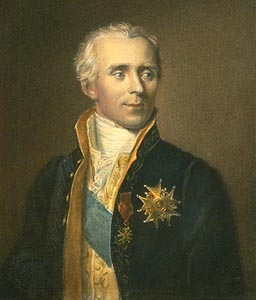
\includegraphics[width=0.5\textwidth]{laplace}
\colc
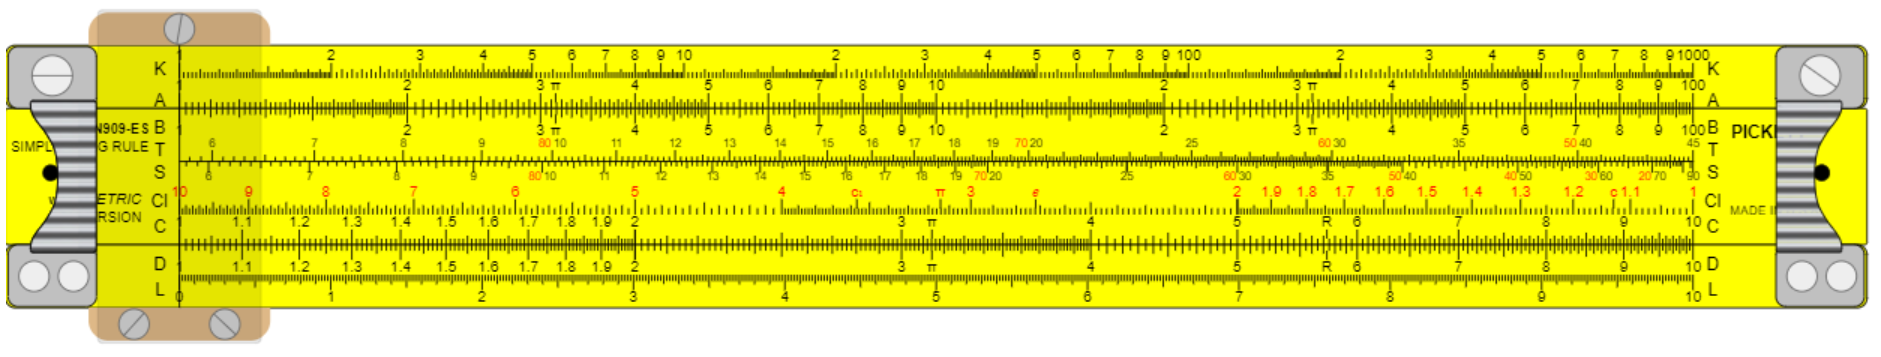
\includegraphics[width=\textwidth]{sliderule}

\centerline{\url{https://www.sliderules.org/}}
\end{frame}


\bfr{Logarithm refresher}
\[
\log_b(a) = c  \Leftrightarrow b^c = a
\]
\begin{align*}
b^{\log_b(a)} &= a\\
\log_b(ac) &= \log_b(a) + \log_b(c)\\
\log_b(a) &= \frac{\log_d(a)}{\log_d(b)} & \frac{a}{b} = \frac{a/d}{b/d}\\
\log_d(b)\log_b(a) &= \log_d(a) & \frac{b}{d}\frac{a}{b} = \frac{a}{d}\\
\log_b(a) &= \frac{1}{\log_a(b)}\\
\log_b(a) &= k\log_d(a) &
\log_{10}(1203248) &\approx 6\\
&&\log_2(1203248) &\approx 20
\end{align*}
\end{frame}


\bfr{Logarithmic scales}
\fig{.7}{linear-log-scales-1.png}

\scriptsize
\cola{0.45}
\bi \li Linear in multiplication
\li Transform the data {\bf or} the axis
\li $\log(x)$ is ambiguous
\ei
\colb{0.55}
\bi
\li Usually preferable to label the axis
\li Why 3.16?
\li Ratios should be shown on log scales.
\ei
\colc
\end{frame}

\bfr{Texas counties, log scale}
\fig{1}{texas-counties-pop-ratio-log-1}
\end{frame}

\bfr{Texas counties, linear scale}
\fig{1}{texas-counties-pop-ratio-lin-1}
\end{frame}

\bfr{Log scales}
\bi
\li
We can think of values greater than 1 as representing multiplications and values less than 1 divisions.
\li
The value 0  can never appear on a log scale: $\log(0) = -\infty$
\li 
It takes infinite divisions to reach zero:  \(1/10/10/10/10/10/10\dots = 0\)
\li
On a log scale, the value 1 is the natural midpoint, similar to the value 0 on a linear scale. 
\li
We can think of values greater than 1 as representing multiplications and values less than 1 divisions.
\ei
\end{frame}


\bfr{Log scales}
\bi
\li
Frequently used when there is a large range in the data:
\bi\li Harris: 4,092,459 \li Loving: 82\ei
\li What if there was a county with 0 inhabitants?
\li This county could not be shown on a logarithmic scale.
\ei
\end{frame}

\bfr{Square root scale}
\bi
\li Can represent zero.
\li Compresses large values and expands small values.
\li But:\bi
\li One step on square root scale does not correspond to addition or multiplication.
\li Hard to place tics. 
\ei
\ei
\fig{.7}{sqrt-scales-1.png}
\end{frame}

\bfr{Square root scale}
\bi
\li Natural axis for areas.
\li Intuitively, the ``breadth'' of an area.
\ei
\fig{1}{northeast-state-areas-1.png}
\end{frame}

\bfr{Curved axes: polar coordinate system}
\fig{1}{polar-coord-1.png}
\end{frame}

\bfr{Curved axes: polar coordinate system}
\bi
\li Useful for periodic data.
\ei
\fig{1}{temperature-normals-polar-1.png}
\end{frame}

\bfr{Curved axes: geospatial data}

\fig{1}{worldmap-four-projections-1.png}
\end{frame}


\bfr{Axis transforms to straighten data}
\end{frame}
\end{document}
